\documentclass{beamer} % "Beamer" is a word used in Germany to mean video projector [  

\usetheme{Berkeley} % Search online for beamer themes to find your favorite or use the Berkeley theme as in this file [ 



\usepackage{color} % It may be necessary to set PCTeX or whatever program you are using to output a  [ pdf instead of a  [ dvi file in order to see color on your screen [ 
\usepackage{graphicx} % This package is needed if you wish to include external image files [ 
\usepackage{hyperref}

\usepackage{amsmath}
\usepackage{amssymb}
\usepackage{amsthm}

\usepackage{amsmath}

\theoremstyle{definition} % See Lesson Three of the LaTeX Manual for more on this kind of "proclamation [ "
\newtheorem*{dfn}{A Reasonable Definition}               

\title{Image Steganography Analysis and Detection}
\author{Subalakshmi Shanthosi S} 
\institute{SSN College of Engineering}
\date{}
% Remove the % from the previous line and change the date if you want a particular date to be displayed; otherwise, today's date is displayed by default [ 

\AtBeginSection[]  % The commands within the following {} will be executed at the start of each section [ 
{
\begin{frame} % Within each "frame" there will be one or more "slides [ "  
\frametitle{Presentation Outline} % This is the title of the outline [ 
\tableofcontents[currentsection]  % This will display the table of contents and highlight the current section [ 
\end{frame}
} % Do not include the preceding set of commands if you prefer not to have a recurring outline displayed during your presentation [ 

\setbeamertemplate{sidebar right}{}
\makeatother

\setbeamertemplate{footline}
{
	\leavevmode%
	\hbox{%
		\begin{beamercolorbox}[wd=.333333\paperwidth,ht=2.25ex,dp=1ex,center]{author in head/foot}%
			\usebeamerfont{author in head/foot}\insertsection
		\end{beamercolorbox}%
		\begin{beamercolorbox}[wd=.333333\paperwidth,ht=2.25ex,dp=1ex,center]{title in head/foot}%
			\usebeamerfont{title in head/foot}\insertsubsection
		\end{beamercolorbox}%
		\begin{beamercolorbox}[wd=.333333\paperwidth,ht=2.25ex,dp=1ex,right]{date in head/foot}%
			\usebeamerfont{date in head/foot}\date[short date]{12-03-1019}\hspace*{2em}
			\insertframenumber{} / \inserttotalframenumber\hspace*{2ex} 
	\end{beamercolorbox}}%
	\vskip0pt%
}
\makeatletter
\setbeamertemplate{navigation symbols}{}
\date[short date]{12-03-2019}

\begin{document}

\begin{frame} 
\titlepage
\end{frame}

\section{What is Image Steganography?} % Since this is the start of a new section, our recurring outline will appear here 

\begin{frame} 
\frametitle{Image Steganography}
 \begin{itemize}
 \item{Steganography is the process of hiding a secret message within a
 larger one in such a way that someone can not know the presence or contents
 of the hidden message }
\end{itemize}
\begin{itemize}
 \item{Aim - To develop a detection system which is capable of detecting the alteration in image both its format and signature thereby predicting the actual type of forged file 
 }
\end{itemize}

\end{frame}

\begin{frame}
\frametitle{Challenges in Forged File Discovery}
 \begin{itemize}
	\item{Images without watermarking as digital signatures can be easily manipulated.}
\end{itemize}
\begin{itemize}
	\item{With the advent of new photo editing software - hiding critical informations are easy and unpercievable }
\end{itemize}
\begin{itemize}
	\item {Task to detect mix of scaled or compressed images as one is difficult}
\end{itemize}
\begin{itemize}
	\item{Incorporating machine learning techniques for feature analysis and decision making  to classify the image to be forged or not  
	}
   \item{Tamper detection to check for change in the file format extension}
\end{itemize}
\end{frame}

\section{Review Papers}
\begin{frame}
\frametitle{Image Steganography Review paper [1]}
\begin{itemize}
	\item{ A detailed literature review on a
		variety of different methods, algorithms, and schemes in image steganography is conducted in order to analyse and
		investigate them
	}
   \item{Methods used:}
   \begin{itemize}
   	\item{Modified LSB(Least Significant Bit) Technique }
   	\item{Modified LSB Technique with AES authentication mechanism  }
   	\item{Steganography approach based on LSB in digital image  }
   	\item{IMStego-Java based Tool with reduced PSNR in conventional LSB approach  }
   \end{itemize}
   \item{ Different Spatial and Transform techniques are realised  }
   \item{Literature review demonstrating the popular steganographic techniques }
\end{itemize}
\end{frame}

\begin{frame}
\frametitle{Image Steganography Based on Modified LSB Substitution Method and Data Mapping [2]}
\begin{itemize}
	\item{Steganographic method working on the principle of Modified LSB Technique with specific intend of reducing the number of 1's in the secret data  }
	\item{Methods:Each pixel value of host image is changed if value of secret bit is 1 otherwise the LSB of each pixel value will remain unchanged }
	\item{Limitation :}
	   \begin{itemize}
	   	\item {Less secure}
	   	\item {Limited pixel quality}
	   \end{itemize}
    \item{State-of-the-art methods in terms of PSNR,SSIM  } 
	\item{Future work:Better data mapping mechanism for reduced storage and computational performance  }
\end{itemize}
\end{frame}

\begin{frame}
\frametitle{Digital Image Steganography Using Modified LSB and AES Cryptography[3]   }
\begin{itemize}
	\item{ This method ensures enhanced security of digital images  }
	\item {Steps involved:}
	\begin{itemize}
	\item{The secret message is transformed to cipher text by AES cryptography [ }
	\item{ The cipher text is hidden inside the image using the modified LSB method }
	\end{itemize}
	\item{Methods:Replacing LSB of cover image with the bits of the concealed message and manipulating the LSB plane of the cover image  }
	\item{Limitation :}
	\begin{itemize}
		\item {Less secure:Easy to decrypt secret message  }
		\item {Less performance  }
	\end{itemize}
	\item{Modified LSB shows improved performance based on PSNR,SSIM metrics  } 
	\item{Future work:Performance Improvement based on storage or computatational time}
\end{itemize}
\end{frame}

\begin{frame}
 \frametitle{Image Steganography with Modified LSB and AES Encryption standards}
	\begin{figure}
		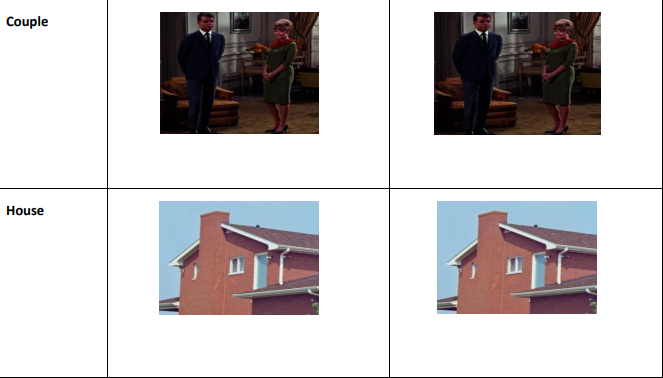
\includegraphics[scale=0.45]{modifiedLSB.png}
		\caption{Image Steganography with Modified LSB and AES Encryption standards}
	\end{figure}
\end{frame}

\begin{frame}
\frametitle{Boundary-based Image Forgery Detection by Fast Shallow CNN[4]   }
\begin{itemize}
	\item{ Network (SCNN) capable of distinguishing the boundaries of
		forged regions from original edges in low resolution images 
		SCNN is designed to utilize the information of chroma and
		saturation  }
	\item{Methods:Based on SCNN:}
	\begin{itemize}
		\item Sliding Windows Detection (SWD) 
		\item Fast SCNN 
	\end{itemize}
	\item {Methodology:}
	\begin{itemize}
		\item{SWD: We start by picking a certain window of an image}
		\item Window is feed into SCNN and compute a confidence score to predict whether it is tampered 
		\item Confidence score and probablity map is maintained   
		\item Then the window slides over and outputs another confidence score   \item After sliding the window through the entire image, a complete probability map is constructed 
    \end{itemize}
\end{itemize}
\end{frame}

\begin{frame}
 \frametitle{Boundary-based Image Forgery Detection by Fast Shallow CNN[4] }
 \begin{itemize}
       \item{Fast SCNN :}
       \begin{itemize}
       	\item Takes entire image as the input  
       	\item Produces feature maps by processing the entire image
			with Conv layers 
		\item Extract feature vectors with dimension from feature maps and feed them into fully-connected layers  
		\item The parameters of Fast SCNN are all trained by SCNN on
			the patch dataset 
		\end{itemize}
	\end{itemize}
\begin{itemize}
	\item{Limitation :}
	\begin{itemize}
		\item {Less secure:Easy to decrypt secret message }
		\item {Less performance  }
	\end{itemize}
	\item{Modified LSB shows improved performance based on PSNR,SSIM metrics  } 
	\item{Future work:Performance Improvement based on storage or computatational time }
\end{itemize}
\end{frame}

\begin{frame}
\frametitle{A Review on Deep Learning based Image Steganalysis [5]   }
\begin{itemize}
	\item{Steganalysis based on deep learning approach  }
	\item{Classified as the following categories:}
	\begin{itemize}
		\item Spatial Image Steganalysis 
		\item JPEG Domain  Steganalysis  
	\end{itemize}
\end{itemize}
\begin{itemize}
	 \item{Deep Learning based Steganalysis  }
	\begin{itemize}
		\item {Spatial Domain Steganography Steganalysis based on Deep Neural Network Design  }
		\begin{itemize}
			\item Spatial Rich model(SRM)  
			\item Steganalysis Based on Fusion Approach 
			\item Steganalysis methods based on Learning Strategy
		\end{itemize}
	    \item{ Jpeg Domain Steganography Steganalysis based on Deep
	    	Learning  }
    	\begin{itemize}
    		\item Convolutional Neural Network(CNN) with 20 layers 
    		\item CNN with 32 layers combined with  SCA-GFR 
    		\item CNN with four 5 x 5 high pass filters, which
    		include a “KV filter”, a “point filter”, and 2 Gabor filters, are
    		used to detect stego noise introduced by JPEG-domain
    		embedding scheme 
    	\end{itemize}
	\end{itemize}
\end{itemize}
\end{frame}

\begin{frame}
\frametitle{A Review on Deep Learning based Image Steganalysis [5]   }
\begin{itemize}
	\item{Limitation and Mitigation:}
\end{itemize}
	\begin{itemize}
		\item {Acquisition and representation of statistical characteristics: Using  Generative Adversarial Network(GAN)  }
		\item {Low payload steganographic image detection: Combination of neural neteork design and various other techniques like training sample creation and learning }
		\item {Generalization of steganalysis: Combine Transfer Learning and Deep Learning}
		\item {Quantitative and locating image steganalysis based on
			deep learning }
	\end{itemize}
\begin{itemize}
	\item{Future work: Challenges resolution by adapting new learning and training sample techniques  }
\end{itemize}
\end{frame}

\begin{frame}
\frametitle{Steganalysis of RGB Images Using Merged Statistical Features of Color Channels[6]  }
\begin{itemize}
	\item The steganalysis process is based on supervised machine learning, utilizing the Support Vector Machine (SVM) binary classifier’s implementation in MATLAB 
	\item Proposed Model:
	\begin{itemize}
        \item{Based on merging features of single color channels into a multi-channel feature set, without consideration to the correlation between color channels  }
        \item{Accuracy of model is evaluated with uncompressed RGB clean image and stego image  }
     \item Feature Selection - Statistical Textural Features
     \begin{itemize}
     	\item Single Channel - Statistical and Traditional Feature Set 
     	\item Multi Channel -  Consists of GLCM features Contrast,Correlation,Energy and Homogeneity, as well as other textural features such as Entropy in the study of textural features of images, and have been used in many steganalysis research works 
     \end{itemize}
	\end{itemize}
\end{itemize}
\end{frame}

\begin{frame}
\frametitle{Single Channel Features in Statistical Textural Features  }
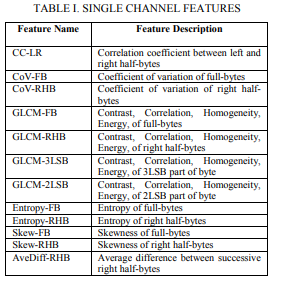
\includegraphics[scale=1.0]{singleChannelFeatures.png}
\end{frame}

\begin{frame}
\frametitle{Steganalysis of RGB Images Using Merged Statistical Features of Color Channels[6]  }
\begin{itemize}
	\item Dataset :  The selected cover image type is uncompressed RGB-BMP, in three channels, without the alpha channel [  Two independent datasets are used, for double validation of the proposed model [  The first validation dataset consists of 1500 clean images in TIFF format with alpha channel, that were downloaded from the Natural Resources Conservation (NRC) image dataset [ 
	\item Dataset : The CALTECH’s birds images dataset [14], which is in a compressed color JPEG format [  A set of 1500 CALTECH images were converted to BMP format and resized to 512 X 512 pixels [  
\end{itemize}
\end{frame}
\begin{frame}
\frametitle{Steganalysis of RGB Images Using Merged Statistical Features of Color Channels[6] [ }
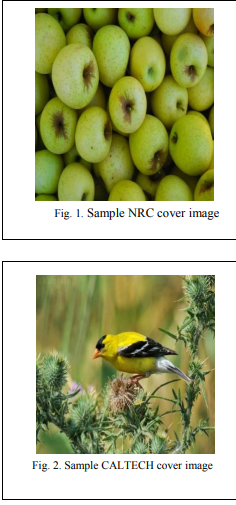
\includegraphics[scale=0.35]{nrcndcaltech.png}
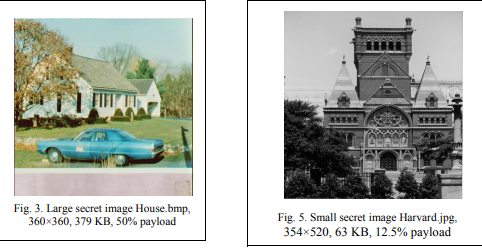
\includegraphics[scale=0.35]{stegImage.png}
\end{frame}

\begin{frame}
\frametitle{Steganalysis of RGB Images Using Merged Statistical Features of Color Channels[6]}
\begin{itemize}
\item Experimental Work:
 \begin{itemize}
 	 	\item Embedding : Secret messages are embedded using Spatial Steganography
 	\begin{itemize}
 	\item Each Channel in each pixel were Embedded with 2 bits or 4 bits by replacing the least significant bits [  For single channel embedding, only the NRC cover images were used, in which the Blue color channel of each pixel was embedded using 2-bpc 
 	\item  The processes of embedding have produced five stego datasets: NRC-LSB2, NRC-LSB4, CALTECH-LSB2, CALTECHLSB4, and NRC-2LSB-Blue  
 \end{itemize}
      \item Features Extraction: Using build in functions of MATLAB 
      \item Classification using SVM Classifier
      \item Evaluation metrics :True Negative(TN),True Positive(TP), False Negative(FN) , False Positive(FP) and Detection Accuracy(DA)  
\end{itemize}
\end{itemize}
\end{frame}

\begin{frame}
\frametitle{Steganalysis of RGB Images Using Merged Statistical Features of Color Channels[6] }
\begin{itemize}
\item Limitation: 
 \begin{itemize}
 	\item Does not apply to compressed images with lossey compression 
 	\item Performance and Storage consideration for Multi channel 
 	\item Capacity of hiding data is low 
 \end{itemize}
 \item Future Work : The proposed steganalysis model can be evaluated using 
 \begin{itemize}
 	\item Lower embedding rates 
 	\item Different media types : audio and video  
 	\item Flexibility to work with transform domain  
 \end{itemize}
 \end{itemize}
\end{frame}

\begin{frame}
\frametitle{Large-Scale JPEG Image Steganalysis Using Hybrid Deep-Learning Framework[7]  }
\begin{itemize}
	\item Deep Learning in Image Steganalysis is still in its initial stage-A generic hybrid deep-learning framework for JPEG steganalysis incorporating the domain knowledge behind rich steganalytic models
	\item Stages in JPEG Steganalysis:
	\begin{itemize}
		\item The first stage is hand-crafted, corresponding to the convolution phase followed by for rich model : 
		\begin{itemize}
            \item 	Quantization phase  
            \item   Truncation phase 
		\end{itemize}
	    \item The second stage is a compound deep-neural network containing multiple deep subnets, in which the model parameters are learned in
		the training procedure  
	\end{itemize}
\end{itemize}
\end{frame}
\begin{frame}
\frametitle{Large-Scale JPEG Image Steganalysis Using Hybrid Deep-Learning Framework[7]  }
\begin{itemize}
		\item Proposed Model:
	\begin{itemize}
		\item{Preliminaries: }
		\begin{itemize}
			\item 	The principal part of CNN is a cascade of alternating convolutional layers, regulation layers (eg. BN layers) and pooling layers  
		\end{itemize}
\end{itemize}
\item Working : 
\begin{itemize}
	\item Each neuron unit receives inputs from a previous layer, performs a dot product with weights and optionally follows it with a nonlinear point-wise activation function 
	\item CNNs can be trained using backpropagation 
\end{itemize}
\item Quantisation and Truncation in Steganalysis:
\begin{itemize}
	\item Convolution with series of kernal to derive varied noise residuals 
	\item Quantisation  
	\item Truncation 
	\item Aggregation  
\end{itemize}
\end{itemize}
\end{frame}

\begin{frame}
\frametitle{Large-Scale JPEG Image Steganalysis Using Hybrid Deep-Learning Framework[7]  }
\begin{itemize}
\item Hybrid Deep Learning Approach :
\begin{itemize}
	\item Takes Decompressed JPEG images and performes Convolution and Quantisation,Truncation
	\item The second stage is a compound deep CNN network in which the model parameters are learned in the training procedure 
\end{itemize}
\item Future Work : 
\begin{itemize}
	\item Incorporation of Adversarial Machine Learning into current hybrid framework  
	\item Exploration of the application of hybrid framework in
	the field of multimedia forensics 
\end{itemize}
\end{itemize}
\end{frame}

\begin{frame}
\frametitle{Large-Scale JPEG Image Steganalysis Using Hybrid Deep-Learning Framework[7]  }

\begin{figure}
	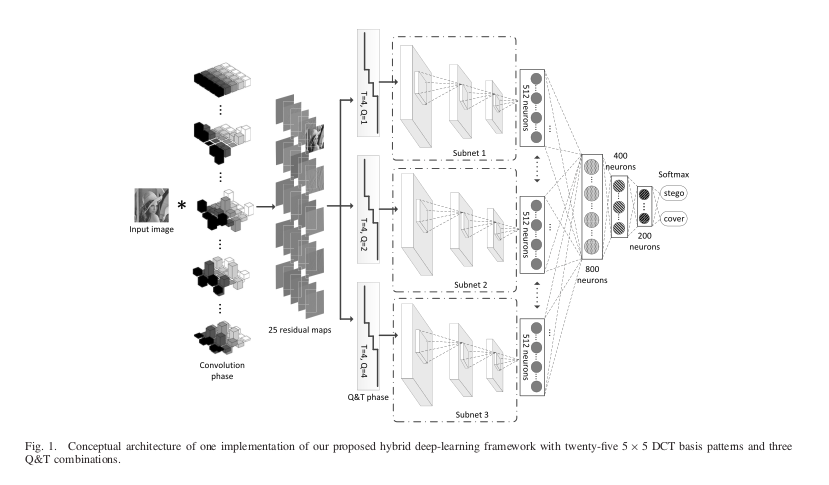
\includegraphics[scale=0.3]{jpegStegAnalysis.png}
	\caption{Hybrid Deep Learning Framework}
\end{figure}
\end{frame}

\begin{frame}
\frametitle{Steganalysis based on Steganography Pattern Discovery[8] }
\begin{itemize}
	\item SPD Approach:
	\begin{itemize}
		\item Evolutionary method Steganalysis to extract the signature of stego images against clean images via fuzzy if–then rules  
		
		\item Blind steganalysis on the discovered knowledge, suitable trained models for steganalysis can be employed and stego images will be detected with high accuracy   
		\item Using SPD, we can predict the type of steganography method from a stego image [  Employing SPD can enhance the approaches, which
		assume that a special steganography method is used 
		\item The effect of SPD before applying steganalysis methods has been investigated by some steganography and steganalysis techniques and it has been validated using some image databases  
		\item The second stage is a compound deep CNN network in which the model parameters are learned in the training procedure 
	\end{itemize}
\end{itemize}
\end{frame}

\begin{frame}
\frametitle{Steganalysis based on Steganography Pattern Discovery[8]  }
\begin{itemize}
	\item Steps carried out in SPD : 
	\begin{itemize}
		\item Image Feature Selection, Two Groups as methods: 
		\begin{itemize}
			\item Filtering :Select feature subsets independently from the learning classifiers and do not include learning 
			\item Wrapping :Wrap around a certain learning algorithm that can
			assess the selected feature subsets in terms of estimated classification errors and then build the final classifiers  
		\end{itemize}
		\item Fuzzy rule generation : Iterative Rule Learning approach, each individual codes one rule and in each iteration of Genetic Algorithm (GA) a new rule is adapted and added to the rule set, iteratively  
	\end{itemize} 
\end{itemize}
\end{frame}

\begin{frame}
\frametitle{The block diagram of Steganography pattern discovery [8]  }
\begin{figure}
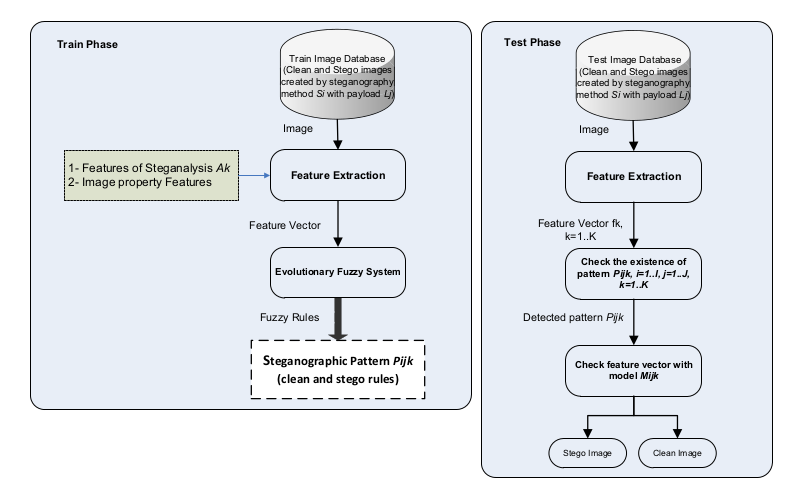
\includegraphics[scale=0.37]{spdBlockDiag.png}
\end{figure}
\end{frame}

\begin{frame}
\frametitle{Steganalysis based on Steganography Pattern Discovery[8]}
\begin{itemize}
	\item Feature vector generation
	\begin{itemize}
	\item 274 dimension Steganalyser 
	\item 324 dimension Feature Vector - First order and second order histograms.
	\item Wavelet based Steganalysis 
	\item 14 dimensional Feature Vector 
	\end{itemize}
\end{itemize}
\end{frame}

\begin{frame}
\frametitle{Steganalysis based on Steganography Pattern Discovery[8]}
\begin{itemize}
	\item Fuzzy rule generation - Evolutionary method searches for a relatively smaller if-then-rules
	\item Certinity Factor for Fuzzy Rules : 
	\begin{itemize}
	    \item Calculate the compatibility of each training sample
	    \item For clean and stego images, calculate the relative sum of the compatibility grades of training samples with rule $R_j$ [ 
	    \item The grade of certainty $CF_j$ for clean images [ 
	\end{itemize}
    \item Evolutionary Fuzzy Algorithm 
    \begin{itemize}
    	\item Initiation.
    	\item Generation. 
    	\item Replacement. 
    	\item Inner Cycle Termination Test. 
    	\item Outer Cycle Termination Test. 
    	\item Weight Adjustement. 
    \end{itemize}
\end{itemize}
\end{frame}

\begin{frame}
\frametitle{Steganalysis based on Steganography Pattern Discovery[8] }
\begin{itemize}
		\item Evolutionary Method : 
		\begin{itemize}
			\item Extracts signature of stego images against clean images using Fuzzy if-then-rules statements 
			\item The Steganalyzer trained to detect only one steganography method at once 
		\end{itemize}
	    \item Limitations : 
	    \begin{itemize}
	    	\item Using Fuzzy rules increases computational complexicity  
	    	\item Only 4 Class Feature Classification - Limited Features  
	    \end{itemize}
\end{itemize}
\end{frame}

\begin{frame}
\frametitle{A Novel Image Steganography Method via Deep Convolutional Generative Adversarial Networks[9]  }
\begin{itemize}
	\item A novel Steganography without Embedding (SWE), which does not need to modify the data of the carrier image, appeared to overcome the detection of machine-learning-based steganalysis algorithms 
	\item SWE method based on deep convolutional generative adversarial networks.
	\begin{itemize}
		\item Generative Adversarial Network (GAN)
		\begin{itemize}
		    \item  GAN and discriminative model [ 
		    \item The henerative model deceives the discriminative model via generated images that appear like real images while the discriminative
		    model judges whether the images are real or unreal. 
		\end{itemize}
		\item Deep Convolutional Generatice Adversarial Network (DGAN)
		\begin{itemize}
		    \item Deep convolutional generative adversarial networks (DCGANs) are an extension of GANs in which the models are deep convolutional
		    networks 
		    \item Currently, GANs are widely used for the following works: 
		    \item Image generation 
		    \item Image restoration
		    \item Image steganography(seldomly), especially SWE  
		\end{itemize}
			\end{itemize}
		\end{itemize}
\end{frame}

\begin{frame}
\frametitle{A Novel Image Steganography Method via Deep Convolutional Generative Adversarial Networks[9] [ }
\begin{figure}
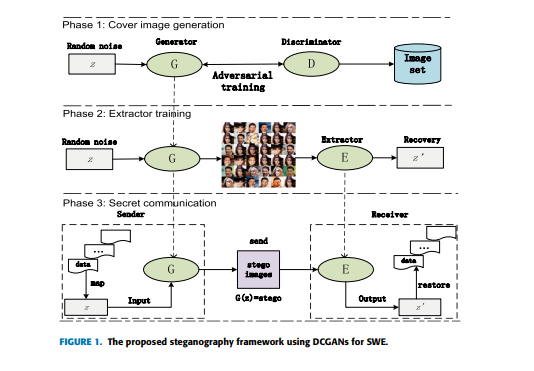
\includegraphics[scale=0.5]{DCGANSWE.png}
\caption{Steganography Framework using DCGAN and SWE.}
\end{figure}
\end{frame}
\begin{frame}
\frametitle{A Novel Image Steganography Method via Deep Convolutional Generative Adversarial Networks[9]}
\begin{itemize}
	\item The Proposed Image Steganography without embedding: 
	\begin{itemize}
		\item Train DCGANs on an image set and obtain generator G after DCGANs convergence.
		\item Train a CNN's model, called the extractor E, based on the recovery errors from a large number of random noise vectors. 
		\item The sender and the receiver hold the network and
		parameters of G and E, respectively. 
	\end{itemize}
   \item Cover Image Generation 
   \begin{itemize}
       \item Secret message is segmented $S_i$ and then map each segment $S_i$
       to noise vector $z_i$ .
       \item Generate a cover image stegoi from the noise vector $z_i$ with the help of DCGANs
   \end{itemize}
 \item Training of the Extractor
  \begin{itemize}
  	\item We design the CNNs, called the extractor E, to recover the
  	secret data from stego images generated by G .  
  	\item Has four convolutional fully connected layer . 
  \end{itemize}
\end{itemize}
\end{frame}

\begin{frame}
\frametitle{A Novel Image Steganography Method via Deep Convolutional Generative Adversarial Networks[9]  }
\begin{figure}
	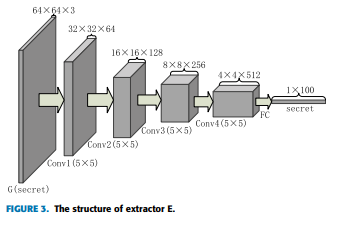
\includegraphics[scale=0.55]{extractorgan.png}
	\caption{The structure of Extractor - E. }
\end{figure}
\end{frame}

\begin{frame}
\frametitle{A Novel Image Steganography Method via Deep Convolutional Generative Adversarial Networks[9] }
\begin{itemize}
    \item  leak-Relu activation function and batch normalization in each layer with no pooling layer or dropout operation   
    \item Afully connected layer is used after last convolutional layer  
    \item Train E to extract information from the generated stego images from G   \item The training procedure of the extractor is,
\end{itemize}
\begin{block}{Formula}
	\begin{equation}
	L(E) = \sum_{i=1}^{n} (z - E(stego)^2)
	\end{equation}
\end{block}
\end{frame}

\begin{frame}
\frametitle{A Novel Image Steganography Method via Deep Convolutional Generative Adversarial Networks[9]  }
\begin{itemize}
	\item  Secret Communication 
	\begin{itemize}
		\item Sender holds the CNNs model G and the corresponding network parameters of G and the receiver holds the CNNs model E and the corresponding network parameters of E 
	\end{itemize}
\end{itemize}
\end{frame}

\section{Reference Papers}

\begin{itemize}
	\item{\textbf{Image Steganography Review paper [1]}, International Journal of Advanced Research in Computer and Communication Engineering(IJARCCE) , Mohammed A  Saleh ,\href{https://ijarcce.com/wp-content/uploads/2018/10/IJARCCE20187910.pdf} {DOI}. }
\end{itemize}

\begin{itemize}
	\item{\textbf{Digital Image Steganography Using Modified LSB and AES Cryptography[2]} ,   International Journal of Computer Science and Network Security(IJCSNS) ,Subhash Panwara , Shreenidhi Damanib , Mukesh Kumar \href{http://www.ijrerd.com/papers/v3-i6/3-IJRERD-C149.pdf}{DOI} [ }
	\end{itemize}
\begin{itemize}
	\item{\textbf{Boundary-based Image Forgery Detection by Fast Shallow CNN
	[3]} , 2018 24th International Conference on Pattern Recognition (ICPR) , Zhongping Zhang , Yixuan Zhang , Zheng Zhou , Jiebo Luo , \href{http://doi [ org/10 [ 1109/ICPR [ 2018 [ 8545074} {DOI} [  }

\end{itemize}

\begin{itemize}
	\item {\textbf{Boundary-based Image Forgery Detection by Fast Shallow CNN [4]  [ } , 2018 24th International Conference on Pattern Recognition (ICPR) , Zhongping Zhang , Yixuan Zhang , Zheng Zhou , Jiebo Luo , \href{https://doi. org/10. 1109/ICPR. 2018. 8545074}{DOI}. }
\end{itemize}

\begin{itemize}
	\item {\textbf{A Review on Deep Learning based Image Steganalysis [5]. } ,  2018 IEEE 3rd Advanced Information Technology, Electronic and Automation Control Conference (IAEAC) ,Yong-he TANG, Lie-hui JIANG, Hong-qi HE, Wei-yu DONG , \href{http://doi. org/10. 1109/IAEAC. 2018. 8577655} {DOI}. }
\end{itemize}
\begin{itemize}
	\item {\textbf{Steganalysis of RGB Images Using Merged Statistical Features of Color Channels[6]} , 2018 11th International Conference on Developments in eSystems Engineering (DeSE) , Zaid I.  Rasool , Mudhafar M.  Al-Jarrah ,Saad Amin , \href{https://doi. org/10. 1109/DeSE. 2018. 00048}{DOI}. }
\end{itemize}
\begin{itemize}
	\item {\textbf{Large-Scale JPEG Image Steganalysis Using
			Hybrid Deep-Learning Framework[7]} ,  IEEE Transactions on Information Forensics and Security , Jishen Zeng  , Shunquan Tan  , Bin Li , Jiwu Huang , \href{https://doi. org/10. 1109/TIFS. 2017. 2779446}{DOI. } }
\end{itemize}
\begin{itemize}
    \item {\textbf{Steganalysis based on steganography pattern
    		discovery[8]} , Journal of Information Security and Applications , Hedieh Sajedi , \href{https://doi.org/10.1016/jjisa. 2016. 04. 001}{DOI. } }
\end{itemize}
\begin{itemize}
	\item{\textbf{A Novel Image Steganography Method via Deep Convolutional Generative Adversarial Networks[9]. }, IEEE Access , Donghui Hu 1 , Liang Wang1 , Wenjie Jiang , Shuli Zheng ,  Bin Li , \href{https://doi.org/10.1109/ACCESS.2018.2852771}{DOI. }}
\end{itemize}
\newpage
\begin{itemize}
     \item {\textbf{Steganography Algorithms Recognition based on Match
     Image and Deep Features Verification[10]. } , Multimedia Tools and Applications Journal ,Xu Xiaoyu ,Sun Yifeng Wu, Jiang , Sun Yi \href{https://doi.org/10.1007/s11042-018-6010-9}{DOI. }}
  
\end{itemize}
\end{document}

